\documentclass[final]{beamer}
\usetheme{RJH}

% references
%\usepackage[bibstyle=authoryear, citestyle=authoryear-comp,%
%  hyperref=auto]{biblatex}
%\bibliography{Biblio}
  
\usepackage[orientation=portrait,size=a0,scale=1.8,debug]{beamerposter}
\usepackage[absolute,overlay]{textpos}
\setlength{\TPHorizModule}{1cm}
\setlength{\TPVertModule}{1cm}

%\usepackage{multicols}
\usepackage{xcolor}

\title{Hazard function models to estimate mortality rates affecting fish populations by maximum likelihood using age data,\\ with application to the sea mullet (Mugil cephalus) fishery on the Queensland coast (Australia)}
\author{Marco Kienzle$^{1,2}$ \\{\small $^{1}$Department of Agriculture and Fisheries, Ecosciences Precinct, Brisbane, QLD 4102, Australia. email: \texttt{Marco.Kienzle@daf.qld.gov.au}\\ $^{2}$ University of Queensland, School of Agriculture and Food Sciences, St. Lucia, QLD 4072, Australia.}
  \vfill
  
\includegraphics[width=15cm, height=5cm]{QG-logo.ps} \hspace{52cm} 
\includegraphics[width=15cm,height=5cm]{UQ-logo.ps}}

%\titlegraphic{
\includegraphics[width=\textwidth,height=.5\textheight]{UQ-logo.ps}}
\footer{}
%\footer{
\includegraphics[width=15cm, height=5cm]{QG-logo.ps} 
\includegraphics[width=15cm,height=5cm]{UQ-logo.ps}}%For more information \texttt{Marco.Kienzle@daf.qld.gov.au} and \texttt{djstgs@bigpond.com}}
\date{}


\begin{document}
\begin{frame}{} 
  \begin{columns}[t]

    %-------------------------------
    % COLUMN 1
    %-------------------------------

    \begin{column}{.47\linewidth}

      %-------------------------------
      % BACKGROUND
      %-------------------------------
      
      %\begin{textblock}{25}(5,10)
      \begin{block}{Background}

        Fisheries management agencies around the world collect age data for the purpose of assessing the status of natural resources in their jurisdiction. Estimates of mortality rates represent a key information to assess the sustainability of fish stocks exploitation. Contrary to medical research or manufacturing where survival analysis is routinely applied to estimate failure rates, survival analysis has seldom been applied in fisheries stock assessment despite similar purposes between these fields of applied statistics.
        
      \end{block}

      %-------------------------------
      % METHOD
      %-------------------------------
      
      %\begin{textblock}{25}(5,10)
      \begin{block}{Method}

        The likelihood function of a sample of age ($S_{k,l}$) was derived for each cohort ($k$) from the hazard function:
        \begin{equation}
          h_{k}(t, \theta) = M + q \ s(t) \ E(t)
          \end{equation}

\begin{equation}
\mathcal{L} = \prod_{k=1}^{n+p-1} \prod_{l=1}^{r_{k}}  \bigl ( \int_{t=a_{k,l}}^{t=a_{k,l+1}} g_{k}(t; \theta) \ dt \bigr ) ^ {S_{k,l}}
\end{equation}

\noindent where

\begin{equation}
\tiny
g_{k}(t; \theta) = \frac{q \ s(t) \ E(t) \times e^{-Mt-q\int_{0}^{t} s(t) \ E(t) \ dt}}{\sum_{l=1}^{r_{k}} \frac{q \ s_{k,l} \ E_{k,l}}{M+q \ s_{k,l} \ E_{k,l}} \bigl ( e^{-M \ a_{k,l}-q\int_{0}^{a_{k,l}}s(t) \ E(t) \ dt} - e^{-M \ a_{k,l}-q\int_{0}^{a_{k,l+1}}s(t) \ E(t) \ dt} \bigr )} 
\end{equation}

        
        %\begin{itemize}
            %\item 60 temperature and rainfall time series from 3 BoM weather stations
        %\end{itemize}
        %\begin{center}
          %\includegraphics[scale=0.8]{MarcoStationLabels.ps}
          %\end{center}
        %\begin{itemize}
            %\item model-based estimates of recruitment ($R$) and spawning stock biomass ($S$)
            %\item multiple linear regression method applied to $\rm{log}(R/S)$
            %\item Beverton\&Holt stock-recruitment model
            %\item model selection using Akaike Information Criteria (AIC)
        %\end{itemize}
      \end{block}

      \begin{block}{Monte Carlo}

        The method was tested with Monte Carlo simulations to assess if it allowed to estimate natural mortality using various sample size (125, 250, 500, ...)
        
        \includegraphics[scale=1.2,angle=-90]{../../Results/Graphics/Estimating-NaturalMortality4PresentationColour.ps}
        
      \end{block}

    \end{column}
    
    %-------------------------------
    % COLUMN 2
    %-------------------------------
    \begin{column}{.47\linewidth}

            % ----------------------------------------------------
      % RESULTS: stepAIC table
      % ----------------------------------------------------
      
      \begin{block}{Monte Carlo (cont.)}

        Estimates of catchability ($q$)
        
        \includegraphics[scale=1.2,angle=-90]{../../Results/Graphics/Estimating-Catchability4PresentationColour.ps}
        
      \end{block}

      \begin{block}{Case study}
        The straddling sea mullet ({\it Mugil cephalus}) is caught along the east coast of Australia from Townsville to roughly the border between New South Wales and Victoria. Analyses of parasites concluded that the bulk of sea mullet caught in Queensland fishery is based on local fish populations and not migrating from New South Wales. A scientific survey samples the Queensland fishery in both estuaries and ocean habitats in order to provide a representative description of this population. Mullet age in the samples varied between 0 and 16 years. Data collected between 2007 and 2014 were used to estimate, for the first time in Australia, the magnitude of natural mortality affecting this stock: it was estimated to equal 0.22 $\pm$ 0.08 year$^{-1}$.
        
      \end{block}

      \begin{block}{Conclusions}

        This likelihood method may well find its place into integrated stock assessment as it provided an efficient method to deal with samples of age data. Applications of survival analysis to fishery data could be expanded further, in particular to derive recruitment estimates using the probabilities estimated by survival analysis and total catch from the fishery.

      \end{block}

      \end{column}


  \end{columns}

  %---------------------------------------
  % REFERENCES
  %---------------------------------------
  
  \begin{block}{Reference}
%    \documentclass[final]{beamer}
\usetheme{RJH}

% references
%\usepackage[bibstyle=authoryear, citestyle=authoryear-comp,%
%  hyperref=auto]{biblatex}
%\bibliography{Biblio}
  
\usepackage[orientation=portrait,size=a0,scale=1.8,debug]{beamerposter}
\usepackage[absolute,overlay]{textpos}
\setlength{\TPHorizModule}{1cm}
\setlength{\TPVertModule}{1cm}

%\usepackage{multicols}
\usepackage{xcolor}

\title{Hazard function models to estimate mortality rates affecting fish populations by maximum likelihood using age data,\\ with application to the sea mullet (Mugil cephalus) fishery on the Queensland coast (Australia)}
\author{Marco Kienzle$^{1,2}$ \\{\small $^{1}$Department of Agriculture and Fisheries, Ecosciences Precinct, Brisbane, QLD 4102, Australia. email: \texttt{Marco.Kienzle@daf.qld.gov.au}\\ $^{2}$ University of Queensland, School of Agriculture and Food Sciences, St. Lucia, QLD 4072, Australia.}
  \vfill
  
\includegraphics[width=15cm, height=5cm]{QG-logo.ps} \hspace{52cm} 
\includegraphics[width=15cm,height=5cm]{UQ-logo.ps}}

%\titlegraphic{
\includegraphics[width=\textwidth,height=.5\textheight]{UQ-logo.ps}}
\footer{}
%\footer{
\includegraphics[width=15cm, height=5cm]{QG-logo.ps} 
\includegraphics[width=15cm,height=5cm]{UQ-logo.ps}}%For more information \texttt{Marco.Kienzle@daf.qld.gov.au} and \texttt{djstgs@bigpond.com}}
\date{}


\begin{document}
\begin{frame}{} 
  \begin{columns}[t]

    %-------------------------------
    % COLUMN 1
    %-------------------------------

    \begin{column}{.47\linewidth}

      %-------------------------------
      % BACKGROUND
      %-------------------------------
      
      %\begin{textblock}{25}(5,10)
      \begin{block}{Background}

        Fisheries management agencies around the world collect age data for the purpose of assessing the status of natural resources in their jurisdiction. Estimates of mortality rates represent a key information to assess the sustainability of fish stocks exploitation. Contrary to medical research or manufacturing where survival analysis is routinely applied to estimate failure rates, survival analysis has seldom been applied in fisheries stock assessment despite similar purposes between these fields of applied statistics.
        
      \end{block}

      %-------------------------------
      % METHOD
      %-------------------------------
      
      %\begin{textblock}{25}(5,10)
      \begin{block}{Method}

        The likelihood function of a sample of age ($S_{k,l}$) was derived for each cohort ($k$) from the hazard function:
        \begin{equation}
          h_{k}(t, \theta) = M + q \ s(t) \ E(t)
          \end{equation}

\begin{equation}
\mathcal{L} = \prod_{k=1}^{n+p-1} \prod_{l=1}^{r_{k}}  \bigl ( \int_{t=a_{k,l}}^{t=a_{k,l+1}} g_{k}(t; \theta) \ dt \bigr ) ^ {S_{k,l}}
\end{equation}

\noindent where

\begin{equation}
\tiny
g_{k}(t; \theta) = \frac{q \ s(t) \ E(t) \times e^{-Mt-q\int_{0}^{t} s(t) \ E(t) \ dt}}{\sum_{l=1}^{r_{k}} \frac{q \ s_{k,l} \ E_{k,l}}{M+q \ s_{k,l} \ E_{k,l}} \bigl ( e^{-M \ a_{k,l}-q\int_{0}^{a_{k,l}}s(t) \ E(t) \ dt} - e^{-M \ a_{k,l}-q\int_{0}^{a_{k,l+1}}s(t) \ E(t) \ dt} \bigr )} 
\end{equation}

        
        %\begin{itemize}
            %\item 60 temperature and rainfall time series from 3 BoM weather stations
        %\end{itemize}
        %\begin{center}
          %\includegraphics[scale=0.8]{MarcoStationLabels.ps}
          %\end{center}
        %\begin{itemize}
            %\item model-based estimates of recruitment ($R$) and spawning stock biomass ($S$)
            %\item multiple linear regression method applied to $\rm{log}(R/S)$
            %\item Beverton\&Holt stock-recruitment model
            %\item model selection using Akaike Information Criteria (AIC)
        %\end{itemize}
      \end{block}

      \begin{block}{Monte Carlo}

        The method was tested with Monte Carlo simulations to assess if it allowed to estimate natural mortality using various sample size (125, 250, 500, ...)
        
        \includegraphics[scale=1.2,angle=-90]{../../Results/Graphics/Estimating-NaturalMortality4PresentationColour.ps}
        
      \end{block}

    \end{column}
    
    %-------------------------------
    % COLUMN 2
    %-------------------------------
    \begin{column}{.47\linewidth}

            % ----------------------------------------------------
      % RESULTS: stepAIC table
      % ----------------------------------------------------
      
      \begin{block}{Monte Carlo (cont.)}

        Estimates of catchability ($q$)
        
        \includegraphics[scale=1.2,angle=-90]{../../Results/Graphics/Estimating-Catchability4PresentationColour.ps}
        
      \end{block}

      \begin{block}{Case study}
        The straddling sea mullet ({\it Mugil cephalus}) is caught along the east coast of Australia from Townsville to roughly the border between New South Wales and Victoria. Analyses of parasites concluded that the bulk of sea mullet caught in Queensland fishery is based on local fish populations and not migrating from New South Wales. A scientific survey samples the Queensland fishery in both estuaries and ocean habitats in order to provide a representative description of this population. Mullet age in the samples varied between 0 and 16 years. Data collected between 2007 and 2014 were used to estimate, for the first time in Australia, the magnitude of natural mortality affecting this stock: it was estimated to equal 0.22 $\pm$ 0.08 year$^{-1}$.
        
      \end{block}

      \begin{block}{Conclusions}

        This likelihood method may well find its place into integrated stock assessment as it provided an efficient method to deal with samples of age data. Applications of survival analysis to fishery data could be expanded further, in particular to derive recruitment estimates using the probabilities estimated by survival analysis and total catch from the fishery.

      \end{block}

      \end{column}


  \end{columns}

  %---------------------------------------
  % REFERENCES
  %---------------------------------------
  
  \begin{block}{Reference}
%    \documentclass[final]{beamer}
\usetheme{RJH}

% references
%\usepackage[bibstyle=authoryear, citestyle=authoryear-comp,%
%  hyperref=auto]{biblatex}
%\bibliography{Biblio}
  
\usepackage[orientation=portrait,size=a0,scale=1.8,debug]{beamerposter}
\usepackage[absolute,overlay]{textpos}
\setlength{\TPHorizModule}{1cm}
\setlength{\TPVertModule}{1cm}

%\usepackage{multicols}
\usepackage{xcolor}

\title{Hazard function models to estimate mortality rates affecting fish populations by maximum likelihood using age data,\\ with application to the sea mullet (Mugil cephalus) fishery on the Queensland coast (Australia)}
\author{Marco Kienzle$^{1,2}$ \\{\small $^{1}$Department of Agriculture and Fisheries, Ecosciences Precinct, Brisbane, QLD 4102, Australia. email: \texttt{Marco.Kienzle@daf.qld.gov.au}\\ $^{2}$ University of Queensland, School of Agriculture and Food Sciences, St. Lucia, QLD 4072, Australia.}
  \vfill
  
\includegraphics[width=15cm, height=5cm]{QG-logo.ps} \hspace{52cm} 
\includegraphics[width=15cm,height=5cm]{UQ-logo.ps}}

%\titlegraphic{
\includegraphics[width=\textwidth,height=.5\textheight]{UQ-logo.ps}}
\footer{}
%\footer{
\includegraphics[width=15cm, height=5cm]{QG-logo.ps} 
\includegraphics[width=15cm,height=5cm]{UQ-logo.ps}}%For more information \texttt{Marco.Kienzle@daf.qld.gov.au} and \texttt{djstgs@bigpond.com}}
\date{}


\begin{document}
\begin{frame}{} 
  \begin{columns}[t]

    %-------------------------------
    % COLUMN 1
    %-------------------------------

    \begin{column}{.47\linewidth}

      %-------------------------------
      % BACKGROUND
      %-------------------------------
      
      %\begin{textblock}{25}(5,10)
      \begin{block}{Background}

        Fisheries management agencies around the world collect age data for the purpose of assessing the status of natural resources in their jurisdiction. Estimates of mortality rates represent a key information to assess the sustainability of fish stocks exploitation. Contrary to medical research or manufacturing where survival analysis is routinely applied to estimate failure rates, survival analysis has seldom been applied in fisheries stock assessment despite similar purposes between these fields of applied statistics.
        
      \end{block}

      %-------------------------------
      % METHOD
      %-------------------------------
      
      %\begin{textblock}{25}(5,10)
      \begin{block}{Method}

        The likelihood function of a sample of age ($S_{k,l}$) was derived for each cohort ($k$) from the hazard function:
        \begin{equation}
          h_{k}(t, \theta) = M + q \ s(t) \ E(t)
          \end{equation}

\begin{equation}
\mathcal{L} = \prod_{k=1}^{n+p-1} \prod_{l=1}^{r_{k}}  \bigl ( \int_{t=a_{k,l}}^{t=a_{k,l+1}} g_{k}(t; \theta) \ dt \bigr ) ^ {S_{k,l}}
\end{equation}

\noindent where

\begin{equation}
\tiny
g_{k}(t; \theta) = \frac{q \ s(t) \ E(t) \times e^{-Mt-q\int_{0}^{t} s(t) \ E(t) \ dt}}{\sum_{l=1}^{r_{k}} \frac{q \ s_{k,l} \ E_{k,l}}{M+q \ s_{k,l} \ E_{k,l}} \bigl ( e^{-M \ a_{k,l}-q\int_{0}^{a_{k,l}}s(t) \ E(t) \ dt} - e^{-M \ a_{k,l}-q\int_{0}^{a_{k,l+1}}s(t) \ E(t) \ dt} \bigr )} 
\end{equation}

        
        %\begin{itemize}
            %\item 60 temperature and rainfall time series from 3 BoM weather stations
        %\end{itemize}
        %\begin{center}
          %\includegraphics[scale=0.8]{MarcoStationLabels.ps}
          %\end{center}
        %\begin{itemize}
            %\item model-based estimates of recruitment ($R$) and spawning stock biomass ($S$)
            %\item multiple linear regression method applied to $\rm{log}(R/S)$
            %\item Beverton\&Holt stock-recruitment model
            %\item model selection using Akaike Information Criteria (AIC)
        %\end{itemize}
      \end{block}

      \begin{block}{Monte Carlo}

        The method was tested with Monte Carlo simulations to assess if it allowed to estimate natural mortality using various sample size (125, 250, 500, ...)
        
        \includegraphics[scale=1.2,angle=-90]{../../Results/Graphics/Estimating-NaturalMortality4PresentationColour.ps}
        
      \end{block}

    \end{column}
    
    %-------------------------------
    % COLUMN 2
    %-------------------------------
    \begin{column}{.47\linewidth}

            % ----------------------------------------------------
      % RESULTS: stepAIC table
      % ----------------------------------------------------
      
      \begin{block}{Monte Carlo (cont.)}

        Estimates of catchability ($q$)
        
        \includegraphics[scale=1.2,angle=-90]{../../Results/Graphics/Estimating-Catchability4PresentationColour.ps}
        
      \end{block}

      \begin{block}{Case study}
        The straddling sea mullet ({\it Mugil cephalus}) is caught along the east coast of Australia from Townsville to roughly the border between New South Wales and Victoria. Analyses of parasites concluded that the bulk of sea mullet caught in Queensland fishery is based on local fish populations and not migrating from New South Wales. A scientific survey samples the Queensland fishery in both estuaries and ocean habitats in order to provide a representative description of this population. Mullet age in the samples varied between 0 and 16 years. Data collected between 2007 and 2014 were used to estimate, for the first time in Australia, the magnitude of natural mortality affecting this stock: it was estimated to equal 0.22 $\pm$ 0.08 year$^{-1}$.
        
      \end{block}

      \begin{block}{Conclusions}

        This likelihood method may well find its place into integrated stock assessment as it provided an efficient method to deal with samples of age data. Applications of survival analysis to fishery data could be expanded further, in particular to derive recruitment estimates using the probabilities estimated by survival analysis and total catch from the fishery.

      \end{block}

      \end{column}


  \end{columns}

  %---------------------------------------
  % REFERENCES
  %---------------------------------------
  
  \begin{block}{Reference}
%    \documentclass[final]{beamer}
\usetheme{RJH}

% references
%\usepackage[bibstyle=authoryear, citestyle=authoryear-comp,%
%  hyperref=auto]{biblatex}
%\bibliography{Biblio}
  
\usepackage[orientation=portrait,size=a0,scale=1.8,debug]{beamerposter}
\usepackage[absolute,overlay]{textpos}
\setlength{\TPHorizModule}{1cm}
\setlength{\TPVertModule}{1cm}

%\usepackage{multicols}
\usepackage{xcolor}

\title{Hazard function models to estimate mortality rates affecting fish populations by maximum likelihood using age data,\\ with application to the sea mullet (Mugil cephalus) fishery on the Queensland coast (Australia)}
\author{Marco Kienzle$^{1,2}$ \\{\small $^{1}$Department of Agriculture and Fisheries, Ecosciences Precinct, Brisbane, QLD 4102, Australia. email: \texttt{Marco.Kienzle@daf.qld.gov.au}\\ $^{2}$ University of Queensland, School of Agriculture and Food Sciences, St. Lucia, QLD 4072, Australia.}
  \vfill
  
\includegraphics[width=15cm, height=5cm]{QG-logo.ps} \hspace{52cm} 
\includegraphics[width=15cm,height=5cm]{UQ-logo.ps}}

%\titlegraphic{
\includegraphics[width=\textwidth,height=.5\textheight]{UQ-logo.ps}}
\footer{}
%\footer{
\includegraphics[width=15cm, height=5cm]{QG-logo.ps} 
\includegraphics[width=15cm,height=5cm]{UQ-logo.ps}}%For more information \texttt{Marco.Kienzle@daf.qld.gov.au} and \texttt{djstgs@bigpond.com}}
\date{}


\begin{document}
\begin{frame}{} 
  \begin{columns}[t]

    %-------------------------------
    % COLUMN 1
    %-------------------------------

    \begin{column}{.47\linewidth}

      %-------------------------------
      % BACKGROUND
      %-------------------------------
      
      %\begin{textblock}{25}(5,10)
      \begin{block}{Background}

        Fisheries management agencies around the world collect age data for the purpose of assessing the status of natural resources in their jurisdiction. Estimates of mortality rates represent a key information to assess the sustainability of fish stocks exploitation. Contrary to medical research or manufacturing where survival analysis is routinely applied to estimate failure rates, survival analysis has seldom been applied in fisheries stock assessment despite similar purposes between these fields of applied statistics.
        
      \end{block}

      %-------------------------------
      % METHOD
      %-------------------------------
      
      %\begin{textblock}{25}(5,10)
      \begin{block}{Method}

        The likelihood function of a sample of age ($S_{k,l}$) was derived for each cohort ($k$) from the hazard function:
        \begin{equation}
          h_{k}(t, \theta) = M + q \ s(t) \ E(t)
          \end{equation}

\begin{equation}
\mathcal{L} = \prod_{k=1}^{n+p-1} \prod_{l=1}^{r_{k}}  \bigl ( \int_{t=a_{k,l}}^{t=a_{k,l+1}} g_{k}(t; \theta) \ dt \bigr ) ^ {S_{k,l}}
\end{equation}

\noindent where

\begin{equation}
\tiny
g_{k}(t; \theta) = \frac{q \ s(t) \ E(t) \times e^{-Mt-q\int_{0}^{t} s(t) \ E(t) \ dt}}{\sum_{l=1}^{r_{k}} \frac{q \ s_{k,l} \ E_{k,l}}{M+q \ s_{k,l} \ E_{k,l}} \bigl ( e^{-M \ a_{k,l}-q\int_{0}^{a_{k,l}}s(t) \ E(t) \ dt} - e^{-M \ a_{k,l}-q\int_{0}^{a_{k,l+1}}s(t) \ E(t) \ dt} \bigr )} 
\end{equation}

        
        %\begin{itemize}
            %\item 60 temperature and rainfall time series from 3 BoM weather stations
        %\end{itemize}
        %\begin{center}
          %\includegraphics[scale=0.8]{MarcoStationLabels.ps}
          %\end{center}
        %\begin{itemize}
            %\item model-based estimates of recruitment ($R$) and spawning stock biomass ($S$)
            %\item multiple linear regression method applied to $\rm{log}(R/S)$
            %\item Beverton\&Holt stock-recruitment model
            %\item model selection using Akaike Information Criteria (AIC)
        %\end{itemize}
      \end{block}

      \begin{block}{Monte Carlo}

        The method was tested with Monte Carlo simulations to assess if it allowed to estimate natural mortality using various sample size (125, 250, 500, ...)
        
        \includegraphics[scale=1.2,angle=-90]{../../Results/Graphics/Estimating-NaturalMortality4PresentationColour.ps}
        
      \end{block}

    \end{column}
    
    %-------------------------------
    % COLUMN 2
    %-------------------------------
    \begin{column}{.47\linewidth}

            % ----------------------------------------------------
      % RESULTS: stepAIC table
      % ----------------------------------------------------
      
      \begin{block}{Monte Carlo (cont.)}

        Estimates of catchability ($q$)
        
        \includegraphics[scale=1.2,angle=-90]{../../Results/Graphics/Estimating-Catchability4PresentationColour.ps}
        
      \end{block}

      \begin{block}{Case study}
        The straddling sea mullet ({\it Mugil cephalus}) is caught along the east coast of Australia from Townsville to roughly the border between New South Wales and Victoria. Analyses of parasites concluded that the bulk of sea mullet caught in Queensland fishery is based on local fish populations and not migrating from New South Wales. A scientific survey samples the Queensland fishery in both estuaries and ocean habitats in order to provide a representative description of this population. Mullet age in the samples varied between 0 and 16 years. Data collected between 2007 and 2014 were used to estimate, for the first time in Australia, the magnitude of natural mortality affecting this stock: it was estimated to equal 0.22 $\pm$ 0.08 year$^{-1}$.
        
      \end{block}

      \begin{block}{Conclusions}

        This likelihood method may well find its place into integrated stock assessment as it provided an efficient method to deal with samples of age data. Applications of survival analysis to fishery data could be expanded further, in particular to derive recruitment estimates using the probabilities estimated by survival analysis and total catch from the fishery.

      \end{block}

      \end{column}


  \end{columns}

  %---------------------------------------
  % REFERENCES
  %---------------------------------------
  
  \begin{block}{Reference}
%    \input{Kienzle-poster.bbl}
    \bibliographystyle{apalike}
    \bibliography{Biblio}
    \nocite{Kienzle2015} % does not display the citation label
%    \nocite{KienzleEtAl2015}
%    \nocite{KienzleEtAl2017}
  \end{block}
  
\end{frame}
\end{document}

    \bibliographystyle{apalike}
    \bibliography{Biblio}
    \nocite{Kienzle2015} % does not display the citation label
%    \nocite{KienzleEtAl2015}
%    \nocite{KienzleEtAl2017}
  \end{block}
  
\end{frame}
\end{document}

    \bibliographystyle{apalike}
    \bibliography{Biblio}
    \nocite{Kienzle2015} % does not display the citation label
%    \nocite{KienzleEtAl2015}
%    \nocite{KienzleEtAl2017}
  \end{block}
  
\end{frame}
\end{document}

    \bibliographystyle{apalike}
    \bibliography{Biblio}
    \nocite{Kienzle2015} % does not display the citation label
%    \nocite{KienzleEtAl2015}
%    \nocite{KienzleEtAl2017}
  \end{block}
  
\end{frame}
\end{document}
